%General Class Template
\documentclass[12pt]{article}
%Packages to load which give you useful commands
\usepackage{amsmath,amsthm}			% want AMS fonts
\usepackage{amssymb}
\usepackage{lastpage}
\usepackage[pdftex]{graphicx}			% for including images
\usepackage{hyperref}				% for links
\usepackage{epstopdf}
\usepackage{setspace}
\usepackage{tikz}
\usepackage{enumerate}
%\doublespacing
\usepackage{fullpage}
% \usepackage{tkz-graph}
% \usetikzlibrary{shapes.geometric}

\tikzstyle{vertex}=[circle, draw, fill=black, inner sep=0pt, minimum size=1pt]
\newcommand{\vertex}{\node[vertex]}

\renewcommand{\O}{\mathcal{O}}
\newcommand{\D}{\mathcal{D}}
\renewcommand{\H}{\mathcal{H}}
\newcommand{\C}{\mathcal{C}}
\newcommand{\I}{\mathcal{I}}
\newcommand{\w}{\textrm{width}}

\newcommand{\N}{\mathbb{N}}
\newcommand{\Z}{\mathbb{Z}}
\newcommand{\Q}{\mathbb{Q}}
\newcommand{\R}{\mathbb{R}}
\newcommand{\makeset}[2]{ \{#1\;|\;#2\} }

\def\mchoose#1#2{\left(\kern-.2em\binom{#1}{#2}\kern-.2em\right)}
%Sets the margins: I like lots of space for text
\textwidth = 7 in
\textheight = 9.5 in
\oddsidemargin = -0.3 in
\evensidemargin = -0.3 in
\topmargin = -0.4 in
\headheight = 0.0 in
\headsep = 0.0 in
\parskip = 0.2in
\parindent = 0.0in

%defines a few theorem-type environments
\newcommand{\hooray}[1]{#1}
\newtheorem{theorem}{Theorem}
\newtheorem{lemma}[theorem]{Lemma}
\newtheorem{corollary}[theorem]{Corollary}
\newtheorem{proposition}[theorem]{Proposition}
\newtheorem{problem}[theorem]{Problem}
\newtheorem{case}[theorem]{Case}
\newtheorem{subcase}[theorem]{SubCase}
\newtheorem{transrule}[theorem]{TransRule}
\newtheorem{branchrule}[theorem]{BranchRule}
\newtheorem{remark}[theorem]{Remark}
\newtheorem{fact}[theorem]{Fact}
\newtheorem{definition}[theorem]{Definition}
\newtheorem*{example*}{Example}
\begin{document}
	{\large  \hfill Math Camp Week 1 Day 4
\hfill
\today}\\

\section*{Rough Outline}
\begin{itemize}
	\item Go over the relevant graphical definitions needed, specifically the coloring definitions.
	\item Define the geometric dual graph, the medial graph, and use the medial graph to construct a link.
	\item Go the other way with the Tait graph.
	\item Throw in a bunch of examples along the way. %Honestly, might just hand draw the examples on the spot 
\end{itemize}
\section*{Definitions/Introduction}
\begin{definition}[Coloring]
	Let $G$ be a graph. Then a proper $k$-coloring of $G$ is a function surjective function $c:V(G)\to [k]$ such that if $u\sim v$ then $c(u)\neq c(v).$ An improper $k-$coloring is where we omit the adjacency condition.
\end{definition}
\begin{example*}
(Use Images)
\end{example*}
\begin{definition}[Medial Graph]
	Let $G$ be a planar graph embedded in the plane in with some planar embedding. Then the \textit{medial graph of $G$ with respect to the embedding}, denoted by $\Gamma(G)$, is the graph whose vertex set is the edge set of $G$, and two vertices in $\Gamma(G)$ are adjacent if, as edges of $G$, they are consecutive edges for some (possibly unbounded) face of $G$. (A \textit{face} of $G$ is a connected region enclosed by some number of edges.)
\end{definition}

\begin{example*}

	

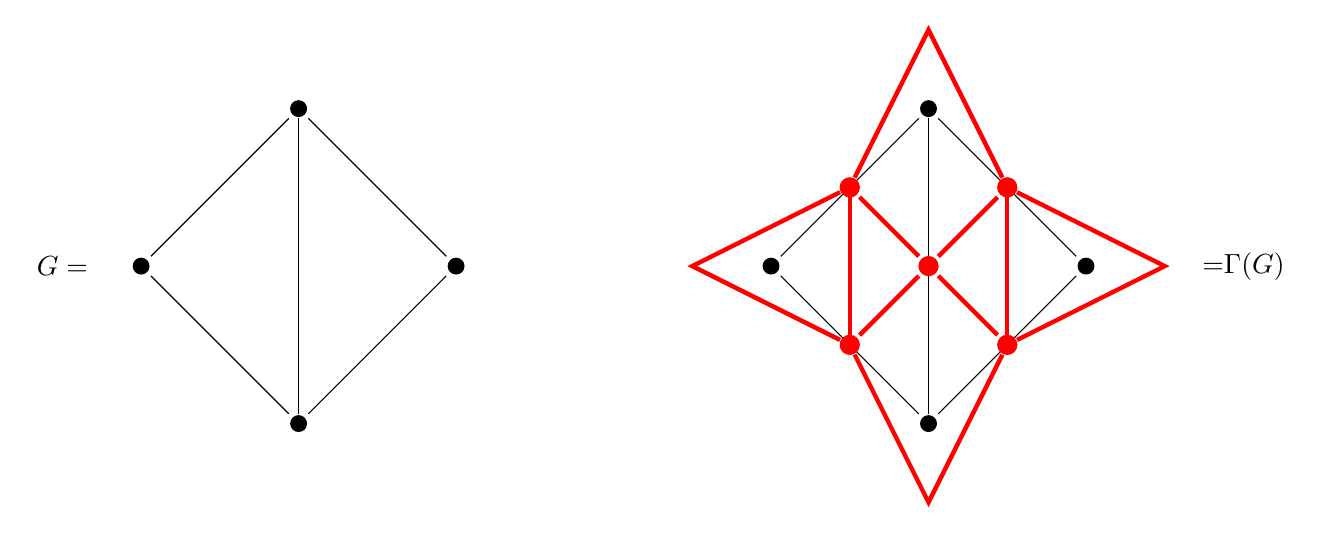
\begin{tikzpicture}
	\node (G) at (-1, 2) {$G =$};
	\node (A) at (2,0) {};
	\node (B) at (0,2) {};
	\node (C) at (4,2) {};
	\node (D) at (2,4) {};
	\draw[fill] (A) circle (.1cm);
	\draw[fill] (B) circle (.1cm);
	\draw[fill] (C) circle (.1cm);
	\draw[fill] (D) circle (.1cm);
	\draw[-] (A) -- (D);
	\draw[-] (A) -- (C);
	\draw[-] (A) -- (B);
%	\draw[-] (B) -- (C);
	\draw[-] (B) -- (D);
	\draw[-] (C) -- (D);
	

	\node (G2) at (14, 2) {=$\Gamma(G)$};
	\node (A2) at (10,0) {};
	\node (B2) at (8,2) {};
	\node (C2) at (12,2) {};
	\node (D2) at (10,4) {};
	\node (E1) at (9,3) {};
	\node (E2) at (10,2) {};
	\node (E3) at (11,3) {};
	\node (E4) at (9,1) {};
	\node (E5) at (11,1) {};
	\draw[fill] (A2) circle (.1cm);
	\draw[fill] (B2) circle (.1cm);
	\draw[fill] (C2) circle (.1cm);
	\draw[fill] (D2) circle (.1cm);
	\draw[-] (A2) -- (D2);
	\draw[-] (A2) -- (C2);
	\draw[-] (A2) -- (B2);
%	\draw[-] (B) -- (C);
	\draw[-] (B2) -- (D2);
	\draw[-] (C2) -- (D2);
	\draw[fill, color = red, ultra thick] (E1) circle (.1cm);
	\draw[fill, color = red, ultra thick] (E2) circle (.1cm);
	\draw[fill, color = red, ultra thick] (E3) circle (.1cm);
	\draw[fill, color = red, ultra thick] (E4) circle (.1cm);
	\draw[fill, color = red, ultra thick] (E5) circle (.1cm);
	\draw[-, color = red, ultra thick] (E2) -- (E1);
	\draw[-, color = red, ultra thick] (E2) -- (E3);
	\draw[-, color = red, ultra thick] (E2) -- (E4);
	\draw[-, color = red, ultra thick] (E2) -- (E5);
	%\draw[-, color = red] (E1) -- (E3);
	%\draw[-, color = red] (E4) -- (E5);
	\draw[-, color = red, ultra thick] (E4) -- (E1);
	\draw[-, color = red, ultra thick] (E5) -- (E3);
	\draw[-,red, ultra thick] (E4)-- (10,-1) --(E5); 
	\draw[-,red, ultra thick] (E4)-- (7,2)--(E1); 
	\draw[-,red, ultra thick] (E1)--(10,5)--(E3); 
	\draw[-,red, ultra thick] (E3) -- (13,2) --(E5); 

\end{tikzpicture}

\end{example*}
\begin{example*}

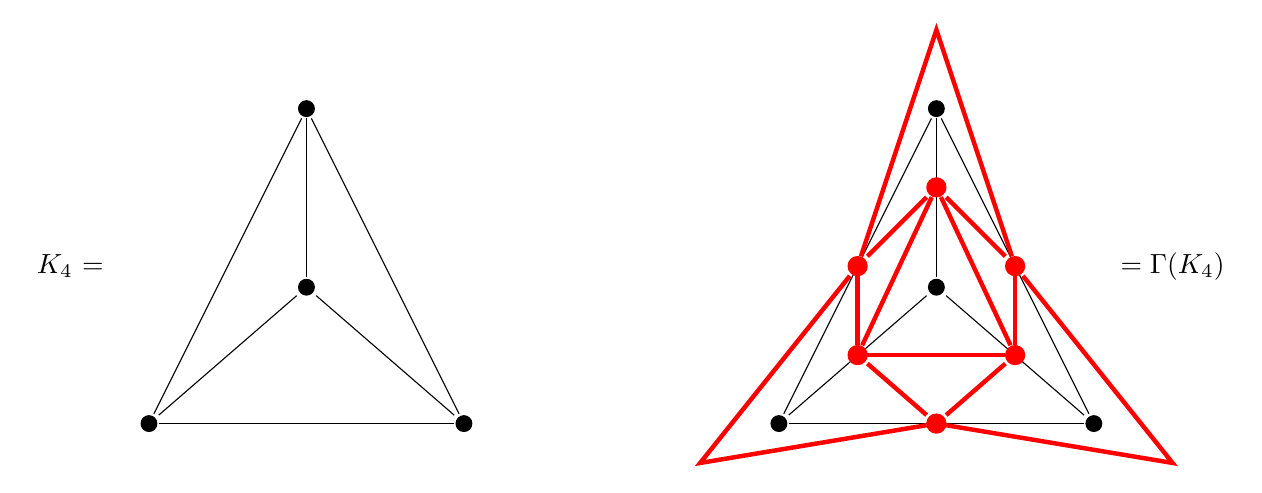
\begin{tikzpicture}
	\node (G) at (-1, 2) {$K_4$ =};
	\node (A) at (2,1.73205) {};
	\node (B) at (0,0) {};
	\node (C) at (4,0) {};
	\node (D) at (2,4) {};
	\draw[fill] (A) circle (.1cm);
	\draw[fill] (B) circle (.1cm);
	\draw[fill] (C) circle (.1cm);
	\draw[fill] (D) circle (.1cm);
	\draw[-] (A) -- (D);
	\draw[-] (A) -- (C);
	\draw[-] (A) -- (B);
	\draw[-] (B) -- (C);
	\draw[-] (B) -- (D);
	\draw[-] (C) -- (D);

\node (G2) at (13, 2) {$=\Gamma(K_4)$};
	\node (A2) at (10,1.73205) {};
	\node (B2) at (8,0) {};
	\node (C2) at (12,0) {};
	\node (D2) at (10,4) {};
	\node (E1) at (10,0) {};
	\node (E2) at (11,.87) {};
	\node (E3) at (9,.87) {};
	\node (E4) at (10,3) {};
	\node (E5) at (9,2) {};
	\node (E6) at (11,2) {};
	\draw[fill] (A2) circle (.1cm);
	\draw[fill] (B2) circle (.1cm);
	\draw[fill] (C2) circle (.1cm);
	\draw[fill] (D2) circle (.1cm);
	\draw[-] (A2) -- (D2);
	\draw[-] (A2) -- (C2);
	\draw[-] (A2) -- (B2);
	\draw[-] (B2) -- (C2);
	\draw[-] (B2) -- (D2);
	\draw[-] (C2) -- (D2);
	\draw[fill, color = red, ultra thick] (E1) circle (.1cm);
	\draw[fill, color = red, ultra thick] (E2) circle (.1cm);
	\draw[fill, color = red, ultra thick] (E3) circle (.1cm);
	\draw[fill, color = red, ultra thick] (E4) circle (.1cm);
	\draw[fill, color = red, ultra thick] (E5) circle (.1cm);
	\draw[fill, color = red, ultra thick] (E6) circle (.1cm);
	\draw[-, color = red, ultra thick] (E2) -- (E1);
	\draw[-, color = red, ultra thick] (E2) -- (E3);
	\draw[-, color = red, ultra thick] (E3) -- (E1);
	\draw[-, color = red, ultra thick] (E2) -- (E4);
	\draw[-, color = red, ultra thick] (E2) -- (E6);
	\draw[-, color = red, ultra thick] (E6) -- (E4);
	\draw[-, color = red, ultra thick] (E3) -- (E5);
	\draw[-, color = red, ultra thick] (E4) -- (E5);
	\draw[-, color = red, ultra thick] (E3) -- (E4);
	\draw[-,red, ultra thick](E1)-- (13,-.5) --(E6); 
	\draw[-,red, ultra thick] (E1)--(7,-.5) --(E5); 
	\draw[-,red, ultra thick](E5)--(10,5)-- (E6); 


\end{tikzpicture}	
\end{example*}
Note that these medial graphs satisfy the property that for every vertex there are exactly 4 edges connected to that vertex. A graph satisfying this property is said to be 4-regular.

\par A medial graph can be thought of as corresponding to some link diagram, without over-under information at the crossings, where the double crossings are the vertices of the medial graph. The following is a procedure to construct a component of the link diagram corresponding to a medial graph:
\begin{enumerate}
	\item Pick some arbitrary vertex $v$ of the medial graph.
	\item Pick some arbitrary edge, $(v,u)$, that connects $v$ to some vertex $u$.
	\item The next edge which will be part of the link is the edge which does not follow or proceed the edge $(v,u)$ in a clockwise orientation around $u$. This edge is well-defined since the medial graph is 4-regular. 
	\item  Repeat the previous step until an edge is repeated. The path of edges determined by this will be the link component.
	\item If, after determining the edges of a link component, there are still edges which are not part of some component, pick one of the remaining edges and one of its end points arbitrarily.
	\item Then begin at the third step starting from the chosen endpoint.
	\item Repeat the fifth step until all edges are part of some link component.
\end{enumerate}

\par This gets us most of the way to where we want to go. All we need to do is determine a way of encoding the over-under information at crossings of the associated link into our graph. To do this, we need the following idea. 
\begin{definition}[Checkerboard Coloring of a Link]
	Let $l$ be an arbitrary link with link projection $L$. Then without loss of generality, assume that the unbounded region of $L$ is considered unshaded
(If the unbounded region were shaded, this would be the checkerboard coloring for a medial link projection of the geometric dual of $G$.) We shade a region $R$ if $R$ shares an edge along its boundary with the boundary of an unshaded region, and similarly we do not shade a region if it shares an edge along its boundary with a shaded region. Then a drawing of $L$ with regions shaded according to this process is called a \textit{checkerboard} coloring of a link. This such coloring is well defined, as we can observe that a region under this definition is unshaded if the region is contained in the intersection of the interior of an even number of link components and is shaded if the region is contained in the intersection of the interior of an odd number of link components.
\end{definition} 
Once we have the checkerboard coloring, we can make a determination of what each crossing looks like locally to encode into our graph. To do this, we will first suppose that to each edge of our graph we associate either of $\pm 1$. From there, using the previously mentioned construction, we can recover the over-under structure of the link in the following manner. If the sign of some edge is 1, which we simplify to $+$, then using the checkerboard coloring the over-under structure of the crossing associated to the edge will look like 
\begin{center}
$	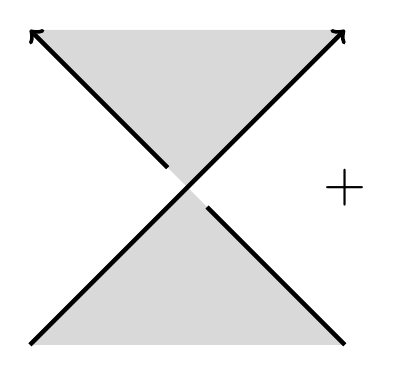
\begin{tikzpicture}
		\fill[gray!30] (0,0) --(2,2) -- (4,0);
		\fill[gray!30] (4,4) --(2,2) -- (0,4);
		\draw[->,ultra thick] (0,0) -- (4,4);
		%\draw[-, ultra thick] (0,4) -- (4,0);
		\draw[<-, ultra thick] (0,4) -- (1.75,2.25);
		\draw[-, ultra thick] (2.25,1.75) -- (4,0);
		\node (+) at (4,2){\scalebox{2}{+}};	
	\end{tikzpicture}$
	\end{center}
Alternatively if the sign of the edge is -1, which we simplify to $-$, then using the checkerboard coloring the over-under structure of the crossing associated to the edge will look like 
	
	\begin{center}
	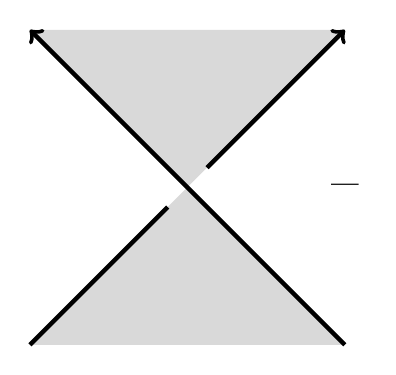
\begin{tikzpicture}
			\fill[gray!30] (0,0) --(2,2) -- (4,0);
		\fill[gray!30] (4,4) --(2,2) -- (0,4);
		\draw[-,ultra thick] (0,0) -- (1.75,1.75);
		\draw[<-, ultra thick] (0,4) -- (4,0);
		%\draw[-, ultra thick] (0,4) -- (1.75,2.25); 
		\draw[->, ultra thick] (2.25,2.25) -- (4,4);
		\node (-) at (4,2){\scalebox{2}{--}};
	\end{tikzpicture}
	\end{center}
This now gives us one way of the correspondence in the case of planar graphs. To go the other way, more precisely than just noting each step was reversible, we need what is known as the Tait graph of a link. The construction of the graph is relatively simple. First, checkerboard color the plane corresponding to the link with the unbounded region uncolored. Then consider each region as a vertex where for each crossing there is a corresponding edge between the two regions it separates. This is called the Tait graph. One can observe that this corresponds exactly to the original graph.

\begin{example*}
(Do a few examples of something going both ways, maybe $K_4$, $K_5$ without an edge, and $C_6$)	
\end{example*}
 
\end{document}